\documentclass[11pt,a4paper]{article}
\usepackage[utf8]{inputenc}
\usepackage[margin=0.8in]{geometry}
\usepackage{tikz}
\usetikzlibrary{shapes.geometric, arrows, positioning, calc, fit, backgrounds}
\usepackage{xcolor}
\usepackage{hyperref}
\usepackage{listings}
\usepackage{enumitem}
\usepackage{tcolorbox}

% Define colors
\definecolor{startcolor}{RGB}{76, 175, 80}
\definecolor{endcolor}{RGB}{244, 67, 54}
\definecolor{processcolor}{RGB}{33, 150, 243}
\definecolor{decisioncolor}{RGB}{255, 193, 7}
\definecolor{actioncolor}{RGB}{156, 39, 176}
\definecolor{issuecolor}{RGB}{255, 87, 34}
\definecolor{fixedcolor}{RGB}{76, 175, 80}

% TikZ styles
\tikzstyle{startstop} = [rectangle, rounded corners, minimum width=3cm, minimum height=1cm, text centered, draw=black, fill=startcolor!30, align=center]
\tikzstyle{process} = [rectangle, minimum width=3cm, minimum height=1cm, text centered, draw=black, fill=processcolor!30, align=center]
\tikzstyle{decision} = [diamond, minimum width=3.5cm, minimum height=1.2cm, text centered, draw=black, fill=decisioncolor!30, aspect=3, align=center, text width=2.5cm]
\tikzstyle{action} = [rectangle, rounded corners, minimum width=3cm, minimum height=1cm, text centered, draw=black, fill=actioncolor!30, align=center]
\tikzstyle{arrow} = [thick,->,>=stealth, rounded corners]
\tikzstyle{state} = [rectangle, rounded corners, minimum width=2.5cm, minimum height=0.8cm, text centered, draw=black, fill=blue!20, align=center, text width=3cm]

\title{\textbf{DecodeShootingAuto v5.0}\\Complete System Documentation\\January 23, 2026 Updates}
\author{FTC Robot Autonomous System}
\date{January 23, 2026}

\begin{document}

\maketitle
\tableofcontents
\newpage

% ============================================================================
\section{Update Summary - January 23, 2026}
% ============================================================================

\subsection{Major Changes Today}

\begin{enumerate}
    \item \textbf{Fixed Intake Timeout Issue} - Added 10-second timeout to prevent infinite hang
    \item \textbf{Fixed Color Sensor Detection} - Implemented live sensor reading (\texttt{readColorNow()})
    \item \textbf{Updated Purple Detection Logic} - Adjusted thresholds based on actual sensor data
    \item \textbf{Created IntakeDebugOpMode} - Standalone testing for intake mechanisms
    \item \textbf{Implemented Smart Intake System} - Pause-for-collection intelligence
    \item \textbf{Fixed Navigation Issue} - Separated Roadrunner trajectory from manual control
\end{enumerate}

\subsection{Current Issues}

\begin{tcolorbox}[colback=issuecolor!10, colframe=issuecolor, title=Known Issues]
\begin{enumerate}[label=\textbf{Issue \arabic*:}]
    \item \textbf{Robot doesn't move forward during SmartIntakeAction}
    \begin{itemize}
        \item Intake and indexing work correctly
        \item Robot reaches intake position successfully
        \item Likely causes:
        \begin{itemize}
            \item Battery/power too low
            \item \texttt{moveSpeed = 0.15} too slow (wheels slipping)
            \item \texttt{drive.setDrivePowers()} not working correctly
        \end{itemize}
        \item \textbf{Next steps}: Increase \texttt{moveSpeed} to 0.3, check battery voltage
    \end{itemize}
    
    \item \textbf{Indexer sometimes requires manual toggle}
    \begin{itemize}
        \item \texttt{isIndexerAtTarget()} may not function correctly
        \item Backup: timeout after 1200ms
    \end{itemize}
\end{enumerate}
\end{tcolorbox}

\newpage
% ============================================================================
\section{Color Sensor Detection Logic}
% ============================================================================

\subsection{Detection Thresholds (Updated)}

Color detection logic was updated based on actual sensor data from testing:

\begin{center}
\begin{tabular}{|l|c|l|}
\hline
\textbf{Parameter} & \textbf{Value} & \textbf{Purpose} \\
\hline
COLOR\_DETECT\_DISTANCE\_CM & 3.5 & Max distance to detect ball \\
Minimum Brightness (R+G+B) & 150 & Avoid scattered light \\
\hline
\multicolumn{3}{|c|}{\textbf{GREEN Detection}} \\
\hline
Condition & \texttt{G > R+30 AND G > B+30} & Green dominates both \\
\hline
\multicolumn{3}{|c|}{\textbf{PURPLE Detection}} \\
\hline
Condition & \texttt{R < G-20 AND R < B-20} & Red is lowest \\
Pattern & G highest, B close to G, R lowest & Based on real data \\
\hline
\end{tabular}
\end{center}

\textbf{Sample Data (Purple ball):}
\begin{verbatim}
Sample 1: R=58,  G=92,  B=79   (G-B=13)
Sample 2: R=135, G=195, B=235  (G-B=40)
Sample 3: R=146, G=215, B=261  (G-B=46)
Sample 4: R=258, G=389, B=500  (G-B=111)
Sample 5: R=141, G=195, B=243  (G-B=48)
\end{verbatim}

Key insight: G-B difference varies widely (13-111), so we don't constrain it.

\newpage
% ============================================================================
\section{SmartIntakeAction State Machine}
% ============================================================================

\subsection{Overview}

The \texttt{SmartIntakeAction} replaces the previous \texttt{ParallelAction} approach with intelligent movement control that \textbf{pauses for ball collection}.

\subsection{State Diagram}

\begin{center}
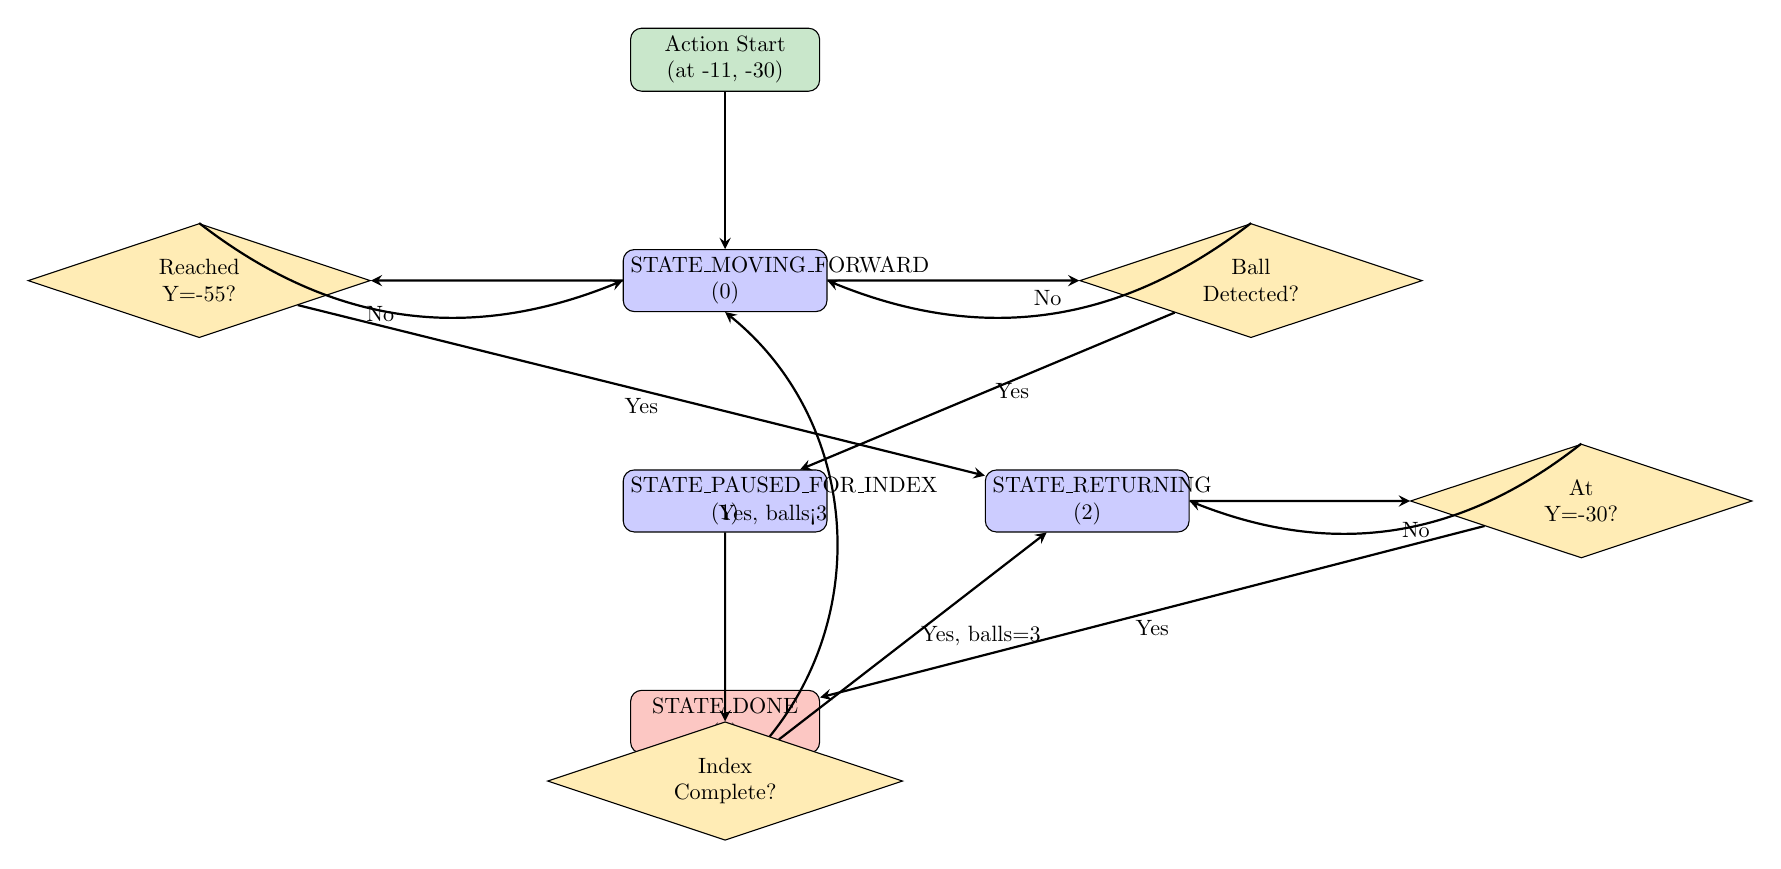
\begin{tikzpicture}[node distance=2.5cm, scale=0.8, transform shape]

% States
\node (start) [startstop] {Action Start\\(at -11, -30)};
\node (forward) [state, below=of start] {STATE\_MOVING\_FORWARD\\(0)};
\node (paused) [state, below=of forward] {STATE\_PAUSED\_FOR\_INDEX\\(1)};
\node (returning) [state, right=of paused] {STATE\_RETURNING\\(2)};
\node (done) [startstop, below=of paused, fill=endcolor!30] {STATE\_DONE\\(3)};

% Decisions
\node (detect) [decision, right=of forward, xshift=1.5cm] {Ball\\Detected?};
\node (target) [decision, left=of forward, xshift=-1.5cm] {Reached\\Y=-55?};
\node (indexdone) [decision, below=of paused, yshift=-0.5cm] {Index\\Complete?};
\node (backhome) [decision, right=of returning, xshift=1cm] {At\\Y=-30?};

% Arrows
\draw [arrow] (start) -- (forward);
\draw [arrow] (forward) -- (detect);
\draw [arrow] (detect) -- node[right] {Yes} (paused);
\draw [arrow] (detect.north) to [bend left=30] node[above] {No} (forward.east);
\draw [arrow] (forward) -- (target);
\draw [arrow] (target) -- node[below] {Yes} (returning);
\draw [arrow] (target.north) to [bend right=30] node[left] {No} (forward.west);
\draw [arrow] (paused) -- (indexdone);
\draw [arrow] (indexdone) to [bend right=45] node[left] {Yes, balls<3} (forward.south);
\draw [arrow] (indexdone) -- node[right] {Yes, balls=3} (returning);
\draw [arrow] (returning) -- (backhome);
\draw [arrow] (backhome) -- node[below] {Yes} (done);
\draw [arrow] (backhome.north) to [bend left=30] node[right] {No} (returning.east);

\end{tikzpicture}
\end{center}

\newpage
\subsection{State Descriptions}

\begin{enumerate}[label=\textbf{STATE \arabic*:}]
    \item \textbf{MOVING\_FORWARD (0)}
    \begin{itemize}
        \item Robot moves slowly forward (Y decreasing)
        \item \texttt{moveSpeed = 0.15} (tunable)
        \item Continuously reads color sensor
        \item Edge detection: EMPTY $\rightarrow$ GREEN/PURPLE triggers
        \item Transitions:
        \begin{itemize}
            \item Ball detected $\rightarrow$ PAUSED\_FOR\_INDEX
            \item Reached Y = -55 $\rightarrow$ RETURNING
            \item 3 balls collected $\rightarrow$ RETURNING
        \end{itemize}
    \end{itemize}
    
    \item \textbf{PAUSED\_FOR\_INDEX (1)}
    \begin{itemize}
        \item Robot \textbf{STOPS MOVEMENT COMPLETELY}
        \item \texttt{drive.setDrivePowers(Vector2d(0, 0))}
        \item Calls \texttt{revolver.indexerNextSlot()}
        \item Waits for indexing (max 1200ms)
        \item Intake keeps running
        \item Transitions:
        \begin{itemize}
            \item Index complete + balls < 3 $\rightarrow$ MOVING\_FORWARD
            \item Index complete + balls = 3 $\rightarrow$ RETURNING
        \end{itemize}
    \end{itemize}
    
    \item \textbf{RETURNING (2)}
    \begin{itemize}
        \item Robot moves back to start (Y = -30)
        \item Faster speed (0.3)
        \item Intake motor OFF
        \item Transitions:
        \begin{itemize}
            \item Within 2" of Y=-30 $\rightarrow$ DONE
        \end{itemize}
    \end{itemize}
    
    \item \textbf{DONE (3)}
    \begin{itemize}
        \item Stops all movement
        \item Returns \texttt{false} to end action
    \end{itemize}
\end{enumerate}

\newpage
% ============================================================================
\section{Complete Autonomous Flow (Updated)}
% ============================================================================

\begin{center}
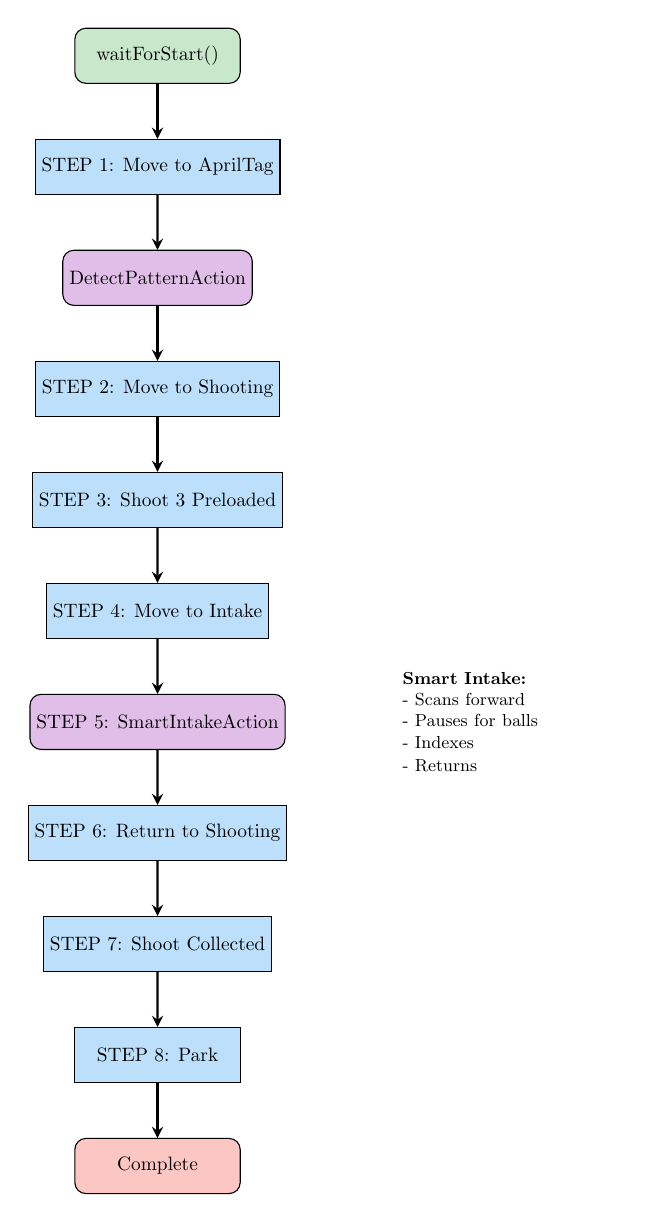
\begin{tikzpicture}[node distance=1cm, scale=0.7, transform shape]

% Nodes
\node (start) [startstop] {waitForStart()};
\node (step1) [process, below=of start] {STEP 1: Move to AprilTag};
\node (detect) [action, below=of step1] {DetectPatternAction};
\node (step2) [process, below=of detect] {STEP 2: Move to Shooting};
\node (step3) [process, below=of step2] {STEP 3: Shoot 3 Preloaded};
\node (step4) [process, below=of step3] {STEP 4: Move to Intake};
\node (step5) [action, below=of step4] {STEP 5: SmartIntakeAction};
\node (step6) [process, below=of step5] {STEP 6: Return to Shooting};
\node (step7) [process, below=of step6] {STEP 7: Shoot Collected};
\node (step8) [process, below=of step7] {STEP 8: Park};
\node (end) [startstop, below=of step8, fill=endcolor!30] {Complete};

% Arrows
\draw [arrow] (start) -- (step1);
\draw [arrow] (step1) -- (detect);
\draw [arrow] (detect) -- (step2);
\draw [arrow] (step2) -- (step3);
\draw [arrow] (step3) -- (step4);
\draw [arrow] (step4) -- (step5);
\draw [arrow] (step5) -- (step6);
\draw [arrow] (step6) -- (step7);
\draw [arrow] (step7) -- (step8);
\draw [arrow] (step8) -- (end);

% Annotations
\node[right=of step5, xshift=1cm, text width=4cm, align=left] {
    \small
    \textbf{Smart Intake:}\\
    - Scans forward\\
    - Pauses for balls\\
    - Indexes\\
    - Returns
};

\end{tikzpicture}
\end{center}

\newpage
% ============================================================================
\section{IntakeDebugOpMode}
% ============================================================================

A standalone opmode for testing intake mechanisms in isolation.

\subsection{Purpose}
Test automatic intake + color sensor + indexer without drivetrain movement.

\subsection{Operation Flow}

\begin{center}
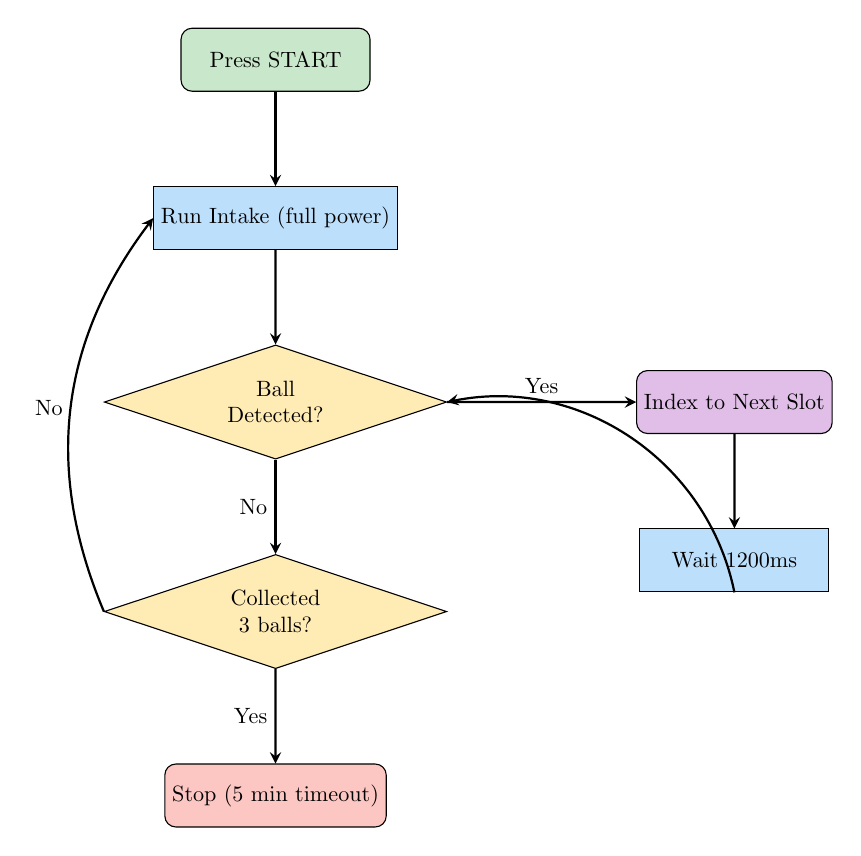
\begin{tikzpicture}[node distance=1.5cm, scale=0.8, transform shape]

\node (start) [startstop] {Press START};
\node (intake) [process, below=of start] {Run Intake (full power)};
\node (scan) [decision, below=of intake] {Ball\\Detected?};
\node (index) [action, right=of scan, xshift=1.5cm] {Index to Next Slot};
\node (wait) [process, below=of index] {Wait 1200ms};
\node (check) [decision, below=of scan] {Collected\\3 balls?};
\node (done) [startstop, below=of check, fill=endcolor!30] {Stop (5 min timeout)};

\draw [arrow] (start) -- (intake);
\draw [arrow] (intake) -- (scan);
\draw [arrow] (scan) -- node[above] {Yes} (index);
\draw [arrow] (scan) -- node[left] {No} (check);
\draw [arrow] (index) -- (wait);
\draw [arrow] (wait.south) to [bend right=45] (scan.east);
\draw [arrow] (check) -- node[left] {Yes} (done);
\draw [arrow] (check.west) to [bend left=30] node[left] {No} (intake.west);

\end{tikzpicture}
\end{center}

\subsection{Telemetry Output}
\begin{itemize}
    \item \texttt{Color}: Current detection (GREEN/PURPLE/EMPTY/UNKNOWN)
    \item \texttt{RGB}: Raw sensor values (R:X G:Y B:Z)
    \item \texttt{Distance}: Distance in cm
    \item \texttt{Balls Collected}: Count / Target
    \item \texttt{Status}: Current action
\end{itemize}

\newpage
% ============================================================================
\section{RevolverSubsystem Color Detection}
% ============================================================================

\subsection{State Machine}

\begin{center}
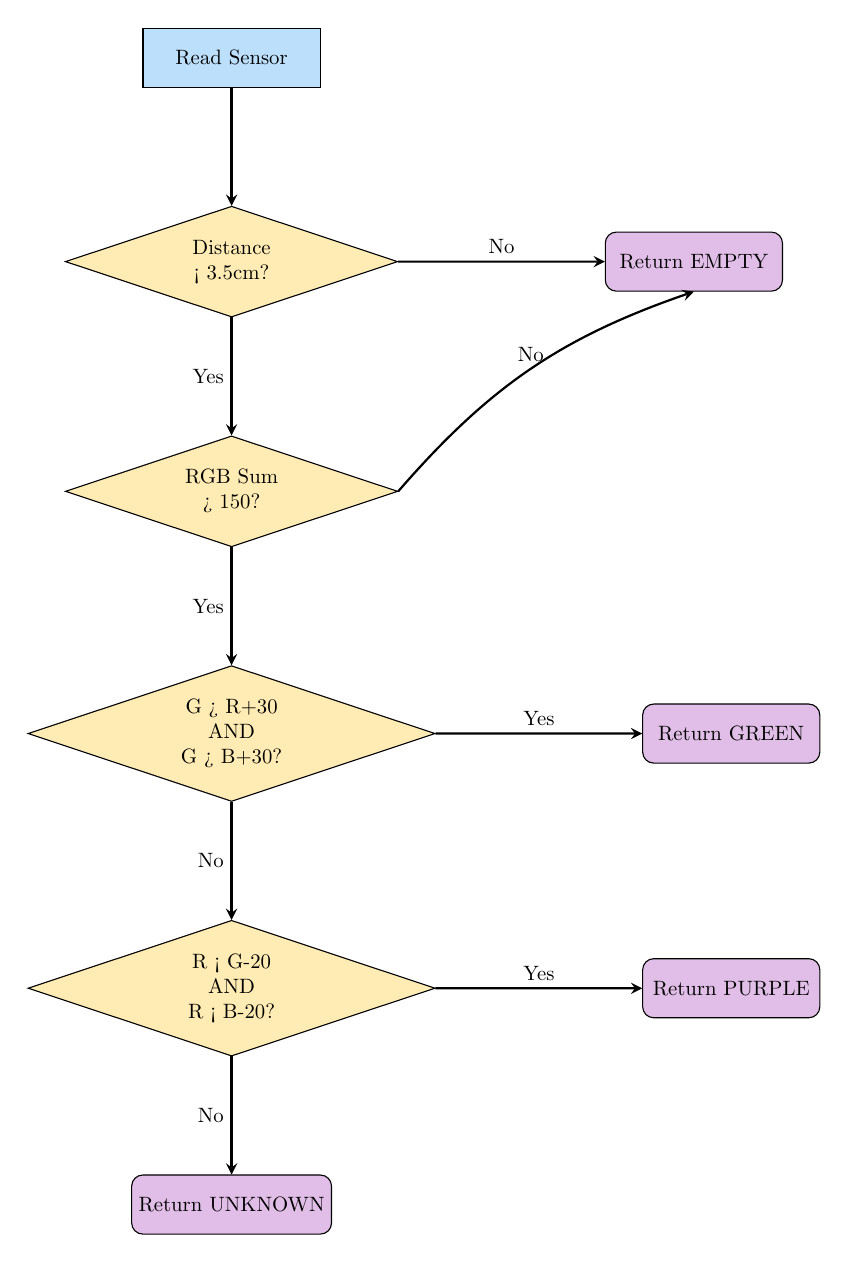
\begin{tikzpicture}[node distance=2cm, scale=0.75, transform shape]

\node (read) [process] {Read Sensor};
\node (dist) [decision, below=of read] {Distance\\< 3.5cm?};
\node (bright) [decision, below=of dist] {RGB Sum\\> 150?};
\node (green) [decision, below=of bright] {G > R+30\\AND\\G > B+30?};
\node (purple) [decision, below=of green] {R < G-20\\AND\\R < B-20?};
\node (det_green) [action, right=of green, xshift=1.5cm] {Return GREEN};
\node (det_purple) [action, right=of purple, xshift=1.5cm] {Return PURPLE};
\node (det_unknown) [action, below=of purple] {Return UNKNOWN};
\node (det_empty) [action, right=of dist, xshift=1.5cm] {Return EMPTY};

\draw [arrow] (read) -- (dist);
\draw [arrow] (dist) -- node[left] {Yes} (bright);
\draw [arrow] (dist) -- node[above] {No} (det_empty);
\draw [arrow] (bright) -- node[left] {Yes} (green);
\draw [arrow] (bright.east) to [bend left=15] node[above] {No} (det_empty.south);
\draw [arrow] (green) -- node[above] {Yes} (det_green);
\draw [arrow] (green) -- node[left] {No} (purple);
\draw [arrow] (purple) -- node[above] {Yes} (det_purple);
\draw [arrow] (purple) -- node[left] {No} (det_unknown);

\end{tikzpicture}
\end{center}

\subsection{Methods}

\begin{itemize}
    \item \texttt{getCurrentColor()} - Returns \textbf{cached} value (updated only when \texttt{update()} called)
    \item \texttt{readColorNow()} - Returns \textbf{live} sensor reading (use in autonomous)
\end{itemize}

\newpage
% ============================================================================
\section{Debugging Timeline}
% ============================================================================

\subsection{Issues Encountered and Fixes}

\begin{tcolorbox}[colback=fixedcolor!10, colframe=fixedcolor, title={Issue 1: Intake Timeout}]
\textbf{Problem:} \texttt{ContinuousIntakeAction} hung forever when no balls detected.\\
\textbf{Cause:} Action always returned \texttt{true}, never exited.\\
\textbf{Fix:} Added 10-second (now 15-second) timeout.
\end{tcolorbox}

\begin{tcolorbox}[colback=fixedcolor!10, colframe=fixedcolor, title={Issue 2: Color Sensor Not Working}]
\textbf{Problem:} No telemetry, balls not detected.\\
\textbf{Cause:} \texttt{getCurrentColor()} returned cached data, but \texttt{update()} never called in autonomous.\\
\textbf{Fix:} Created \texttt{readColorNow()} method for live reading.
\end{tcolorbox}

\begin{tcolorbox}[colback=fixedcolor!10, colframe=fixedcolor, title={Issue 3: False GREEN Detection}]
\textbf{Problem:} Sensor detected GREEN from scattered light.\\
\textbf{Cause:} Distance threshold too high (5cm), no brightness minimum.\\
\textbf{Fix:} 
\begin{itemize}
    \item Reduced distance to 3.5cm
    \item Added minimum brightness check (RGB sum > 150)
\end{itemize}
\end{tcolorbox}

\begin{tcolorbox}[colback=fixedcolor!10, colframe=fixedcolor, title={Issue 4: Purple Not Detected}]
\textbf{Problem:} Most purple ball readings showed UNKNOWN.\\
\textbf{Cause:} Logic required \texttt{|G - B| < 45}, but real data showed 13-111 range.\\
\textbf{Fix:} Simplified to \texttt{R < G-20 AND R < B-20} (R is always lowest).
\end{tcolorbox}

\begin{tcolorbox}[colback=fixedcolor!10, colframe=fixedcolor, title={Issue 5: No Synchronization}]
\textbf{Problem:} Robot completed trajectory without checking if balls collected.\\
\textbf{Cause:} \texttt{ParallelAction} ran independently.\\
\textbf{Fix:} Created \texttt{SmartIntakeAction} with pause-for-collection.
\end{tcolorbox}

\begin{tcolorbox}[colback=fixedcolor!10, colframe=fixedcolor, title={Issue 6: Wrong Navigation}]
\textbf{Problem:} Robot went toward goal instead of intake position.\\
\textbf{Cause:} \texttt{MOVING\_TO\_START} state used simple proportional control.\\
\textbf{Fix:} Use Roadrunner trajectory (\texttt{moveToIntakeStart}), removed \texttt{MOVING\_TO\_START} state.
\end{tcolorbox}

\newpage
% ============================================================================
\section{System Parameters Reference}
% ============================================================================

\subsection{Autonomous Constants}

\begin{center}
\begin{tabular}{|l|c|l|}
\hline
\textbf{Parameter} & \textbf{Value} & \textbf{Description} \\
\hline
\multicolumn{3}{|c|}{\textbf{Timing (ms)}} \\
\hline
SHOOTER\_SPINUP\_MS & 1000 & Shooter warm-up time \\
KICKER\_EXTEND\_MS & 600 & Kicker ejection duration \\
KICKER\_RETRACT\_MS & 400 & Kicker retraction duration \\
INDEXER\_SETTLE\_MS & 500 & Indexer stabilization time \\
INTAKE\_PAUSE\_MS & 1200 & Wait for indexer slot creation \\
\hline
\multicolumn{3}{|c|}{\textbf{Power Levels}} \\
\hline
SHOOTER\_POWER & 0.4 & Shooter motor power \\
INTAKE\_POWER & 1.0 & Intake motor power \\
\hline
\multicolumn{3}{|c|}{\textbf{Smart Intake}} \\
\hline
moveSpeed & 0.15 & Forward speed during scan \\
returnSpeed & 0.3 & Speed when returning \\
startY & -30 & Intake start position \\
endY & -55 & End of intake path \\
MAX\_ACTION\_TIME\_MS & 15000 & Timeout (15 seconds) \\
\hline
\multicolumn{3}{|c|}{\textbf{Color Detection}} \\
\hline
COLOR\_DETECT\_DISTANCE\_CM & 3.5 & Max detection distance \\
Min Brightness & 150 & RGB sum threshold \\
Green dominance & +30 & G must exceed R,B by 30 \\
Purple (R is lowest) & -20 & R must be 20 below G,B \\
\hline
\end{tabular}
\end{center}

\newpage
% ============================================================================
\section{Recommended Next Steps}
% ============================================================================

\subsection{To Fix: Robot Not Moving Forward}

\begin{enumerate}
    \item \textbf{Check Battery Voltage}
    \begin{itemize}
        \item Low battery $\rightarrow$ motors can't overcome friction
        \item Add telemetry: \texttt{voltageSensor.getVoltage()}
    \end{itemize}
    
    \item \textbf{Increase moveSpeed}
    \begin{itemize}
        \item Current: 0.15
        \item Try: 0.3 or 0.4
        \item Edit in FTC Dashboard (it's in \texttt{SmartIntakeAction})
    \end{itemize}
    
    \item \textbf{Verify setDrivePowers}
    \begin{itemize}
        \item Add telemetry in \texttt{STATE\_MOVING\_FORWARD}
        \item Log: currentY, moveSpeed, ballsCollected
        \item Check if \texttt{drive.setDrivePowers()} is actually being called
    \end{itemize}
    
    \item \textbf{Test Manual Control}
    \begin{itemize}
        \item Create simple test: \texttt{drive.setDrivePowers(new PoseVelocity2d(new Vector2d(0, -0.3), 0))}
        \item If this doesn't work, issue is with \texttt{setDrivePowers()} itself
    \end{itemize}
\end{enumerate}

\subsection{To Improve: Indexer Reliability}

\begin{enumerate}
    \item Monitor \texttt{isIndexerAtTarget()} return value
    \item Log indexer position during indexing
    \item If it never returns true:
    \begin{itemize}
        \item Check encoder connection
        \item Verify \texttt{targetPosition} is set correctly
        \item May need to use timeout only
    \end{itemize}
\end{enumerate}

\subsection{Future Enhancements}

\begin{itemize}
    \item \textbf{Dynamic Speed Adjustment}: Slow down further when ball detected
    \item \textbf{Multi-pass Collection}: If < 3 balls, make second pass
    \item \textbf{Vision-based Navigation}: Use camera to locate balls
    \item \textbf{Adaptive Thresholds}: Auto-calibrate color sensor based on ambient
\end{itemize}

\end{document}
